\section{Methods}
\label{ch:ReactionModelsMethods}

To develop the reaction model variants, we assumed mass-action kinetics for all biochemical interactions, leading to ordinary differential equation (ODE) models with 7 states and 12 (10 for the Viral Ub model variant) kinetic parameters. The reaction model schematics (Figure \ref{figure:ReactionModelSchemes}) show all the possible bindings that can occur during motor complex formation. The model variant "Viral Ub" assumes competition between capsid-bound and cellular ubiquitin (Ub) chains for the zinc finger domain of HDAC6. In contrast, the "Symmetric" and "Asymmetric" model variants assume that cellular ubiquitin chains assist with motor binding to HDAC6, both for myosin and dynein motors in the "Symmetric", and only for myosin in the "Asymmetric" model variant. Detailed equations of these models are described in Appendix \ref{appendix:reactionModelsEquations}.

For each set of parameters and initial conditions considered, we simulated the reaction model for 2 hours of system time using the MATLAB ODE solver odeSD \cite{gonnet2012specialized}, such that the protein interactions lead to a steady-state distribution of the molecular species. Then, we used the reaction models' myosin and dynein motor complex abundances (in more detail described in Appendix \ref{appendix:reactionModelsEquations}) at the end of the simulation to predict average capsid breakage probabilities with an interpolated version of the corresponding simulation results for the mass-spring model (Figure \ref{figure:MassSpringInterpolation}).

\begin{figure}
\begin{center}
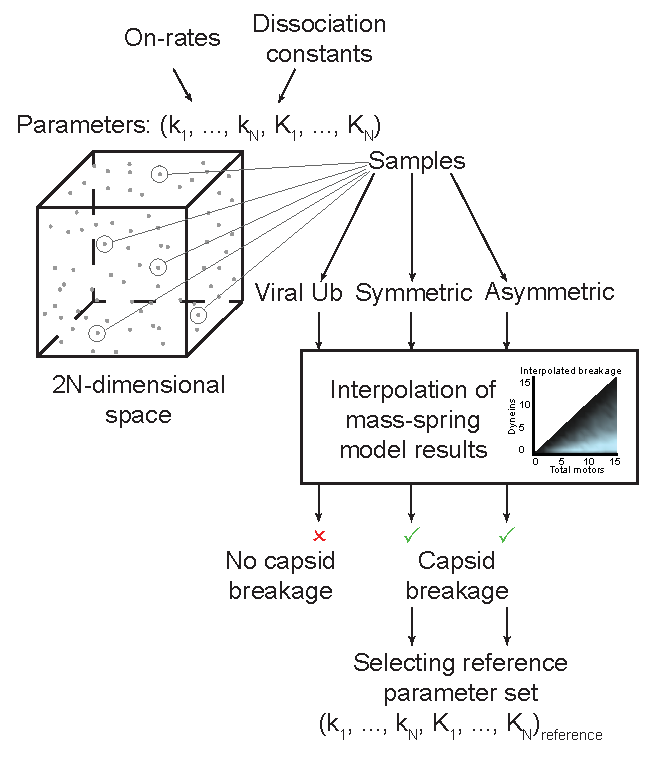
\includegraphics[width=0.80\textwidth, trim={0cm 0cm 0cm 0cm}, clip]{D_chapters/2_ReactionModel/SamplingSchematic copy.pdf}
\caption[Selection of reaction rates reference sets for HDAC6 complex formation models]%
{Selection of reaction rates reference sets for HDAC6 complex formation models. \par
We widely sampled the reaction rates around literature reported values of reaction rates and simulated our models. We used an interpolation of the Mass-Spring model results for average numbers of motor recruitment to determine the expected capsid breakage in the system. "Viral Ub" model variant failed to achieve capsid breakage for any combination of reaction rates. This allowed us to reject the hypothesis that virally carried Ub serves as an interface for binding between M1 capsid protein and HDAC6. For "Symmetric" and "Asymmetric" models we used predicted capsid breakage probabilities to choose reaction rates reference parameter sets, which allow to achieve high breakage and stay close to the literature starting point. 
}
\label{figure:samplingSchematic}
\end{center}
\end{figure}

To optimize reaction rate parameters (Figure \ref{figure:samplingSchematic}), we initially simulated each reaction model variant 100’000 times with fixed median values of initial concentrations and reaction rate constants sampled log normally in the range of $\pm$ 5 orders of magnitude around values reported in the literature (Appendix Table \ref{table:ReactionModelParameters}). These simulation results were then averaged for a single viral particle, and used to compute capsid breakage probabilities using our interpolated mass-spring model results (Figure \ref{figure:MassSpringInterpolation}). The "Viral Ub" variant failed to recruit enough motors to generate any capsid breakage for any combination of reaction rates. Therefore, we focused on the "Symmetric" and "Asymmetric" models.

For both variants, the distribution of capsid breakages showed four modes (Figure \ref{figure:BreakageModesRatesSelection}). Many rate combinations led to zero breakage because the models failed to recruit any motors. The next mode appeared at around 8\% breakage, where the models recruited about 1 myosin motor and 1-2 dynein motors. The next mode capped out at about 50\% breakage, with recruitment of 5-6 myosins, but very low numbers of dyneins, which corresponds to the ‘no dyneins’ case in the mass-spring model. The last mode yielded up to 80-90\% breakage; while sparsely populated, it was able to recruit about 7 myosins and 1-2 dyneins. Since we know that in the experiments capsid breakage depends on both myosins and dyneins, we chose this group for further analysis.

\begin{figure}
\begin{center}
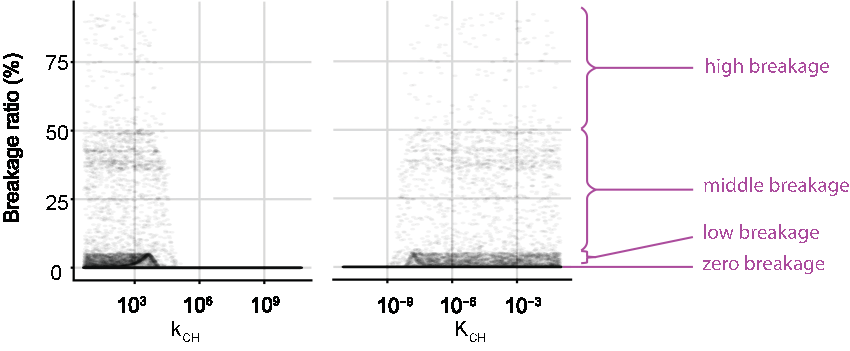
\includegraphics[width=0.95\textwidth, trim={0cm 0cm 0cm 0cm}, clip]{D_chapters/2_ReactionModel/ratesSelection.pdf}
\caption[Breakage ratio modes]%
{Breakage ratio modes observed after  wide sampling around approximate values available in the literature. We optimize the reaction rates using high breakage mode, because it manages to efficiently recruit both myosin and dynein motors.}
\label{figure:BreakageModesRatesSelection}
\end{center}
\end{figure}

Next, we introduced a cost function to evaluate points in this group. It penalizes distance of reaction parameter values from literature values as well as low capsid breakage probability:

\begin{equation}
\begin{split}
C = \sum_{i} \big| \log_{10} \big( \frac{k^i}{k^i_{literature}} \big) \big| +
\sum_{i} \big| \log_{10} \big( \frac{K^i}{K^i_{literature}} \big) \big| + \\
\big| \log_{10} \big( \frac{\%}{\%_{max}} \big) \big|
\end{split}
\end{equation}

where $k^i$ is an on rate, $K^i$ is a dissociation constant, and $\%$ is a capsid breakage probability. Because literature parameter values were of the same order of magnitude (approximately $10^6$ for on rates and $10^{-6}$ for dissociation constants), we did not introduce extra weight coefficients. We selected the parameter point with minimal value of the cost function as reference point.

To compare the performance of "Symmetric" and "Asymmetric" model variants (Figures \ref{figure:densitiesRC}, \ref{figure:densitiesRCsupplementary}), we sampled the concentrations (20’000 times), reaction rates (20’000 times), and both together (40’000 times). Concentrations were sampled uniformly between 50\% and 150\%, and log-normally in $\pm$1 orders of magnitude of the value reported in proteomics experiments (proteomicsDB \cite{schmidt2018proteomicsdb}). Reaction rates were sampled log-uniformly around the reference value in $\pm$1 orders of magnitude, or log-normally around the reference value with a SD of 0.1.

To examine the influence of each individual parameter on the capsid breakage probability, we simulated the model variants with all but one parameter fixed. The free parameter was sampled log-uniformly 20’000 times for concentrations between 50\% and 150\% of the value reported in proteomics experiments (proteomicsDB \cite{schmidt2018proteomicsdb}), and log-uniformly 30’000 times for reaction rate constants around the reference value in $\pm$5 orders of magnitude.

Experimental perturbations, when possible, were translated into model perturbations by changing either reaction rate constants or initial concentrations of reactants (Appendix Table \ref{table:ReactionModelUncoatingNumbers}). We simulated each perturbation 20’000 times similarly to the unperturbed system, with initial concentrations sampled as above and rate constants sampled log-normally around the reference value in $\pm$1 order of magnitude, except for the experiment-specific perturbed parameters or initial conditions, which were sampled in the modified ranges as specified in Appendix Table \ref{table:ReactionModelUncoatingNumbers}.

siRNA for Dynactin2 prevented the binding of dynactin and reduced the amount of available dynein to 1/10 of the norm. Ciliobrevin D, which inhibits the dynein motor activity, stopped the motors from walking, but not from binding; we simulated that case as control, but then assumed zero active dyneins for computing the breakage probability. siRNAs for myosin10 affected the amount of available myosin by reducing it to 1/10 of the norm. siRNAs for myosin9 were not modeled given that experiments showed little effect on the breakage probability. ML-9 and Blebbistatin cases were not simulated as they correspond to zero effective myosins, which, according to the mass-spring model, fails to generate breakage. For the HDAC6 $\Delta$DMC MEF cell line, we assumed an increase of the dissociation constant for HDAC6-dynein binding by a factor of 1000. The HDAC6 KO MEF cell line and siRNA HDAC6 had initial concentrations of HDAC6 reduced to 1/100 and 1/10 of the norm, respectively. The HDAC6 ZnFm (W1116A) MEF cell line had the dissociation constant of HDAC6-Ub binding increased by a factor 1000. We assumed that Cytochalasin D and Nocodazole, which affect actin and tubulin polymerization, reduced the amount of available cytoskeletal scaffolding to 1/10 and 1/100 of the norm, respectively. Importazole is a selective inhibitor of the nuclear transport receptor importin-beta and prevents nuclear import of NLS-containing proteins \cite{soderholm2011importazole}. MG132 is a proteasome inhibitor, leading to misfolded proteins accumulation in the cell and to a depletion of free cellular ubiquitin chains that are no longer recycled during proteasomal degradation of those proteins; therefore, we assumed a reduction in Ub concentration to 1/10 of the norm.

An alternative and, perhaps more biologically reasonable approach to model the domain deletion from HDAC6 would be to remove dynein motors and Ub from the simulation entirely. However, doing so in our ODE reaction model leads to the simulation becoming unstable, and ideally requires additional model modifications, making comparisons between the different reaction models difficult. Modifying reaction rates in contrast, allows us to account for random effects of unspecific binding while keeping the model simple and deterministic.

For the M1 binding signal perturbations, we used H1N1 M1 (and its "restored" virus version H3N2 M1 A218T) as a control, and H2N2 M1 (and its "restored" virus version H1N1 M1 T218A) as a perturbation that increases the HDAC6-capsid dissociation constant by a multiplication factor. We used the average M1 binding signal for the H1N1 M1 T218 mutant and H3N2 WT (Figure \ref{figure:M1ReactionModel}), and fitted a corresponding value of binding to capsid breakage in our individual parameter perturbation experiments (Figure \ref{figure:sampledTrajectories}). The final multiplication factor values were 14.6 for the "Asymmetric" and 23.7 for the "Symmetric" model variant.

For the virus infectivity perturbations, we considered pH1N1 ko/ki WT to be a control, H3N2 ko/ki WT, corresponding to M1-HDAC6 binding dissociation constant being increased by the multiplication factor above, pH1N1 ko/ki ZnF mutant to have an increased ofHDAC6-Ub dissociation constant by a factor of 1000, and H3N2 ko/ki ZnF mutant as both.
